%\documentclass[12pt]{report}
%
%% some macros
%% Here, you can define your own macros. Some examples are given below.

\newcommand{\R}[0]{\mathds{R}} % real numbers
\newcommand{\Z}[0]{\mathds{Z}} % integers
\newcommand{\N}[0]{\mathds{N}} % natural numbers
\newcommand{\C}[0]{\mathds{C}} % complex numbers
\newcommand{\bm}[1]{{\boldsymbol{{#1}}}} % vector
\newcommand{\mat}[1]{{\boldsymbol{{#1}}}} % matrix

\newcommand{\E}[1]{\mathbb{E}_{#1}} % Expectation
\newcommand{\Pd}[1]{\mathbb{P}_{#1}} % Probability Distribution

%%%%%%%%%%%%%%%%%%%%%%%%%%%%%%%%%%%%%%%%%%
% University Assignment Title Page 
% LaTeX Template
% Version 1.0 (27/12/12)
%
% This template has been downloaded from:
%%%%%%%%%%%%%%%%%%%%%%%%%%%%%%%%%%%%%%%%%
%----------------------------------------------------------------------------------------
%	PACKAGES AND OTHER DOCUMENT CONFIGURATIONS
%----------------------------------------------------------------------------------------

\usepackage[nottoc,notlot,notlof]{tocbibind}
\usepackage[T1]{fontenc}
%\usepackage{hyperref}
\usepackage{indentfirst}
\usepackage{amsmath}
\usepackage{amssymb}
\usepackage{graphicx}
\usepackage{subcaption}
\usepackage{geometry}
 \geometry
 {
     a4paper,
     left=25mm,
     right=25mm,
     top=30mm,
     bottom=30mm,
 }

% \usepackage[a4paper,hmargin=2.8cm,vmargin=2.0cm,includeheadfoot]{geometry}
\usepackage{textpos}
\usepackage{natbib} % for bibliography
%\usepackage{tabularx,longtable,multirow,subfigure,caption}
\usepackage{fncylab} %formatting of labels
\usepackage{fancyhdr} % page layout
\usepackage{url} % URLs
\usepackage[english]{babel}
%\usepackage{dsfont}
\usepackage{epstopdf}
\usepackage{backref} % needed for citations
\usepackage{array}
\usepackage{latexsym}
\usepackage[pdftex,pagebackref,hypertexnames=false,colorlinks]{hyperref} % provide links in pdf
 
\hypersetup{pdftitle={},
  pdfsubject={}, 
  pdfauthor={},
  pdfkeywords={}, 
  pdfstartview=FitH,
  pdfpagemode={UseOutlines},% None, FullScreen, UseOutlines
  bookmarksnumbered=true, bookmarksopen=true, colorlinks,
    citecolor=black,%
    filecolor=black,%
    linkcolor=black,%
    urlcolor=black}
 
\usepackage[all]{hypcap}
\frenchspacing

\DeclareMathOperator{\tr}{tr}
%
%\begin{document}

\chapter{Literature Review}

This section shall discuss the currently existing datasets and models relating to visual speech recognition (VSR)
This shall be explored in both the space of two dimensional images and three dimensional scans of speaking subjects, the current successes in these fields and the current issues which are faced in progressing these areas of research forwards.

\section{Current Lip Reading Models and Datasets}

In recent years the problem of VSR, also know as lip reading, has seen huge advances due to the availability of new datasets and the use of Deep Learning models \cite{Chung2016, Chung2017, Shillingford2018}.
This section shall discuss the progresses which have already been made in this field and the datasets publicly available on which to train such models.
Current lip reading models, to the best of the author's knowledge, all make use of 2D temporal data such as videos by evaluating the frames of the video, using this information to make a prediction of the word, or words, which were spoken in the sequence.

However in reality, humans who are able to lip read also have access to three dimensional data due to our depth perception, which is not well represented in 2D video frames; thus is can be hypothesised that some information captured by 3D temporal scans of speaking subjects can also be used for speech prediction.
Unlike 2D temporal data, 3D temporal data (3D video), requires multiple cameras to record simultaneously, which in turn requires synchronisation between the cameras, increasing the complexity of the system beyond simply having multiple cameras.
The data must then be processed to produce the final product, whether this is in the form of video with depth information or more complex 3D scans \cite{Li2017}.

\subsection{Datasets}
There currently exists multiple labelled video datasets which can be used for traditional VSR; here 'traditional' refers to using 2D temporal data.
Datasets such as GRID \cite{Cooke2006}, LRW \cite{Chung2016}, LRS \cite{Chung2017} and LSVSR \cite{Shillingford2018} have been constructed by compiling the video data from various sources, each with an increasing vocabulary and dataset size.

\subsubsection{Controlled Conditions Datasets}
The GRID dataset was released in 2006 \cite{Cooke2006} and contains 34,000 samples from 34 speakers, each with 1000 sentences.
Based on previous work using the coordinate response measure (CRM) \cite{Bolia2000}, the corpus uses sentences with a fixed grammar: <command:4>, <colour:4>, <preposition:4>, <letter:25>, <number:10>, <adverb:4>, with a total vocabulary of 51 words.
Aside from the restricted vocabulary size in comparison to more recent datasets, the primary limiting factor of the GRID dataset is that all data was captured directly for the use of the dataset and so, models trained on this dataset have learnt on controlled conditions, something not found in the desired wider applications of VSR.

\subsubsection{In The Wild Datasets}
To build larger datasets more suited for deep learning models, the following are commonly built with "in the wild" data, meaning that the original videos have not been captured with the intention of being used for this dataset, while the data collected for the datasets is preprocessed such that it is suited for the task.
Variations in lighting, angles, speakers and a wide vocabulary are common, this does however make the datasets more challenging to learn from, but the models are no longer as bias to controlled conditions.

LRW and LRS are both comprised of content from BBC broadcasts \cite{Chung2016, Chung2017} allowing for a far larger corpus size of 500 words for LRW and over 6000 words for LRS.
Both of datasets are captured and processed with the same pipeline (Figure \ref{fig:LRW_Pipeline}) summarised as follows. 

\begin{figure}[h]
    \centering
        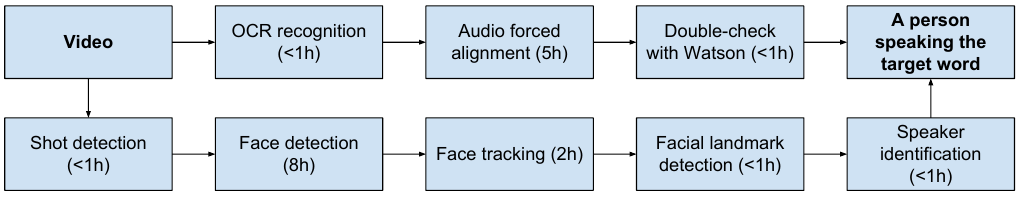
\includegraphics[width=0.95\textwidth]{figures/lrw_pipeline.png}
    \caption{LRW Dataset Pipeline \cite{Chung2016}}\label{fig:LRW_Pipeline}
\end{figure}

Firstly, as the text transcripts are broadcast as bitmaps, optical character recognition (OCR) \cite{Buehler2009} is used to obtain the text spoken in the video, the audio and text are then aligned per frame using the HTK toolkit \cite{Woodland1995}.
The quality of these predictions are validated with the use of the commercial IBM Watson Speech to Text converter.

Secondly, face detection and tracking are used so that the frame can be cropped to feature the subject's mouth at the centre.
To achieve this, a histogram of oriented gradients based (HOG-based) detection algorithm \cite{King2009} is used on all video frames to detect faces, see left hand side of Figure \ref{fig:LRW_Face_Detection}.
A Kanade-Lucas-Tomasi (KLT) feature tracker is also applied to the frames, where both the HOG and KLT overlap (see centre of Figure \ref{fig:LRW_Face_Detection}), it is assumed to be tracking the face correctly.
To identify mouth position, facial landmarks are then used using an ensemble of regression trees method from \cite{Kazemi2014}, see the right of Figure \ref{fig:LRW_Face_Detection}.

\begin{figure}[h]
    \centering
        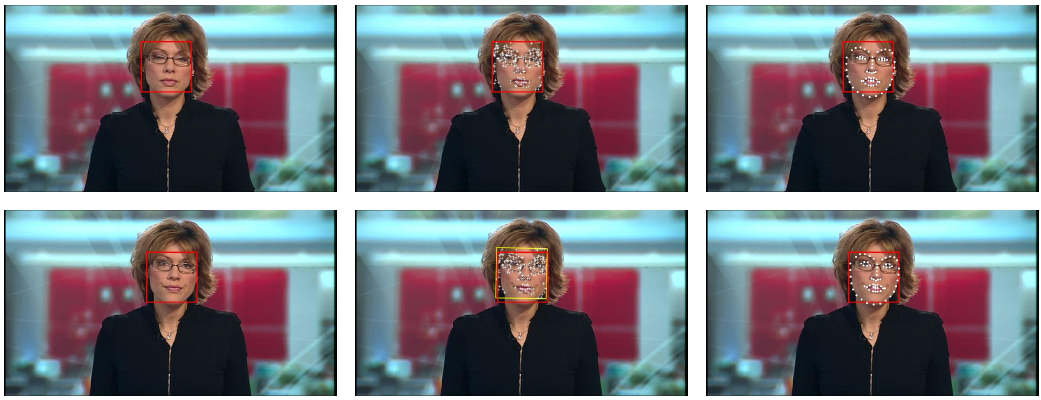
\includegraphics[width=0.99\textwidth]{figures/lrw_face_detection.png}
    \caption{LRW Face Detection and Tracking \cite{Chung2016}}\label{fig:LRW_Face_Detection}
\end{figure}

As multiple faces can appear at any one time, it is assumed that the speaker will be the only subject with a moving mouth.
Assuming that the lip movements fall within a frequency range, the Fourier transform is applied to the openness of the mouth defined by the distance between top and bottom lip from the facial landmarks.
A support vector machine (SVM) is then trained on the frequency spectrum to classify who is speaking in each frame.
The frames are then cropped around the relevant speaker, an example of a sample from the dataset is shown in Figure \ref{fig:LRW_One_Second}.

\begin{figure}[h]
    \centering
        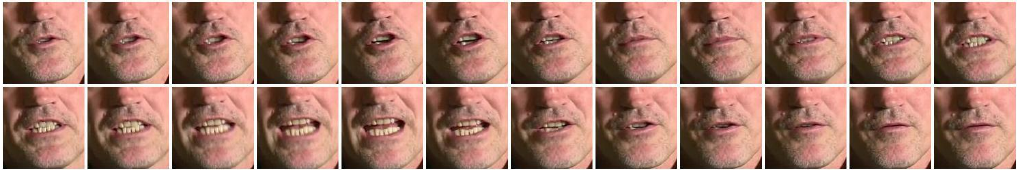
\includegraphics[width=0.99\textwidth]{figures/lrw_one_second.png}
    \caption{LRW Dataset Sample: 24 frames of a subject saying \textit{`about'} \cite{Chung2016}}\label{fig:LRW_One_Second}
\end{figure}

LSVSR is a dataset published by DeepMind and Google which makes use of the huge amount of videos on YouTube \cite{Shillingford2018}, resulting in a total length of 3886 hours of training data.
Unlike LRW or LRS, LSVSR aligns phonemes to frames, as opposed to words or characters.
The pre-processing steps are similar as in LRW and LRS, although the alignment is performed with the algorithm laid out in previous work by DeepMind \cite{Liao2013}.

\subsubsection{3D Datasets} \label{3D Datasets}
To the best of the author's knowledge, there are currently only two datasets with 3D temporal data which could be appropriate for training lip reading models, neither of which have been captured with the intention of being used for VSR.

The first of which is LRW-3D \cite{Tzirakis2019} which has been captured from four subjects, two native English speakers and two non-native to increase variability in the dataset.
The subjects have been captured speaking the corpus used in the LRW dataset \cite{Chung2016}, a vocabulary of 500 words.
The resulting dataset comprises of 660 seconds of 3D meshes and audio per subject.
The dataset is not comprised of full sentences but would be appropriate for word-level lip reading, however a total duration of 660 seconds is likely to be too short for a deep learning model to train effectively.
The dataset had also not been officially published at the time of this report.

The second is the VOCASET \cite{Cudeiro2019}, an unlabelled dataset captured from 6 male and 6 female subjects.
Each subject was recorded speaking 40 sequences, each ranging from 3 to 5 seconds, resulting in a total time of 30 minutes.
The recorded 3D meshes are registered to the FLAME model \cite{Li2017}, a statistical 3D facial mesh with around 5000 vertices, an example sample from the dataset can be seen in Figure \ref{fig:VOCASET_example}.
Unlike the LRW-3D dataset, the sequences are grammatically correct sentences, chosen to maximise phonetic diversity.
This makes the VOCASET appropriate for creating a model for sentence-level lip reading, similarly to LRW-3D, 30 minutes of training data is likely to be a limiting factor when training a deep learning model.

\begin{figure}[h]
    \centering
    \begin{subfigure}[b]{0.19\textwidth}
        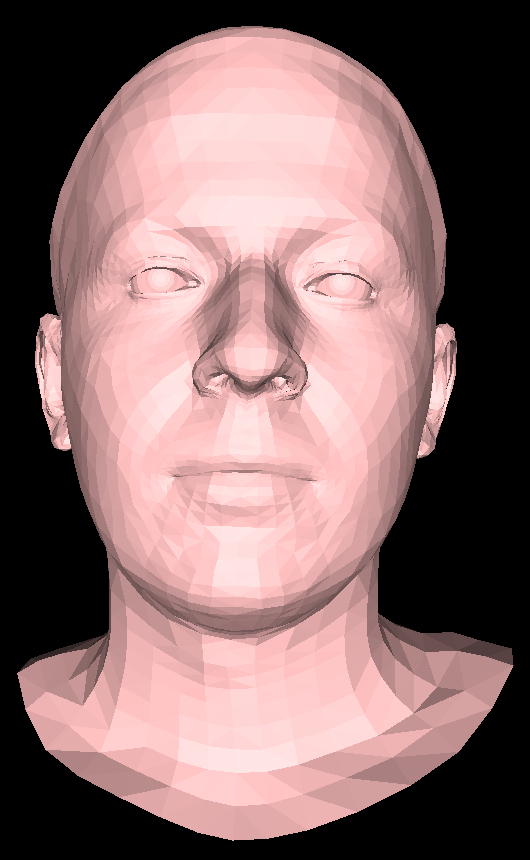
\includegraphics[width=\textwidth]{figures/voca_exp/vocaset_exp1.png}
    \end{subfigure}
    \begin{subfigure}[b]{0.19\textwidth}
        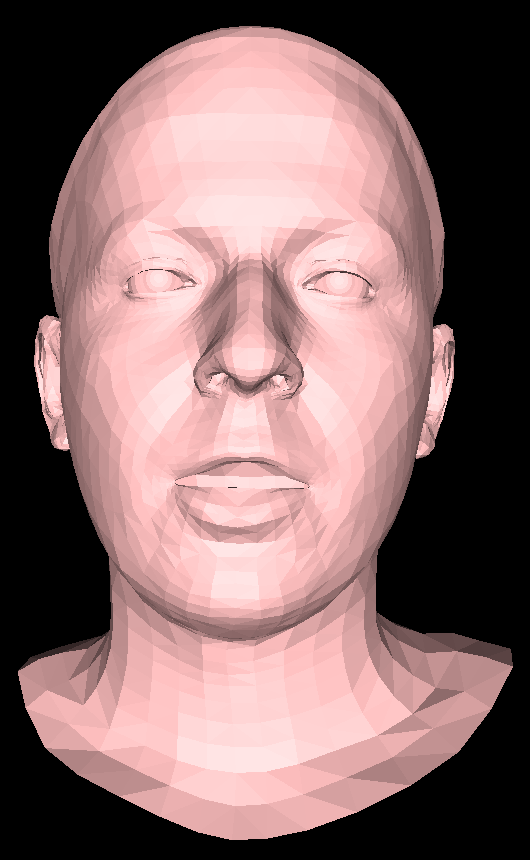
\includegraphics[width=\textwidth]{figures/voca_exp/vocaset_exp2.png}
    \end{subfigure}
    \begin{subfigure}[b]{0.19\textwidth}
        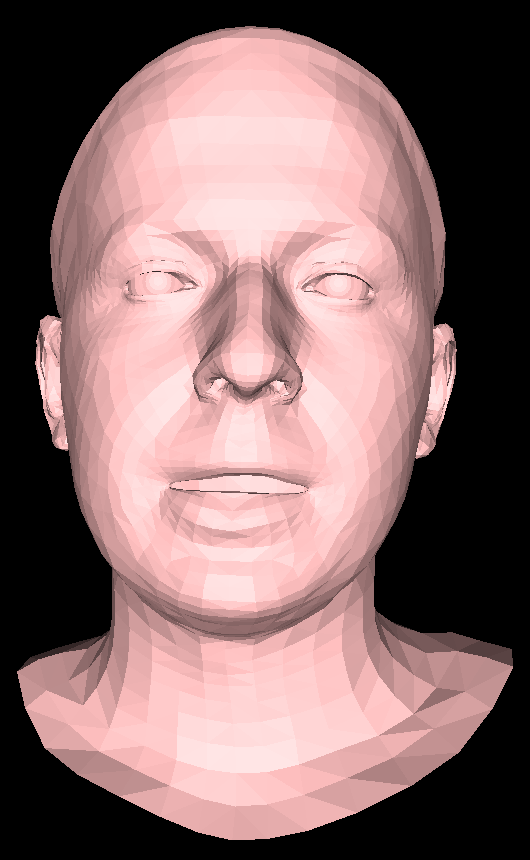
\includegraphics[width=\textwidth]{figures/voca_exp/vocaset_exp3.png}
    \end{subfigure}
    \begin{subfigure}[b]{0.19\textwidth}
        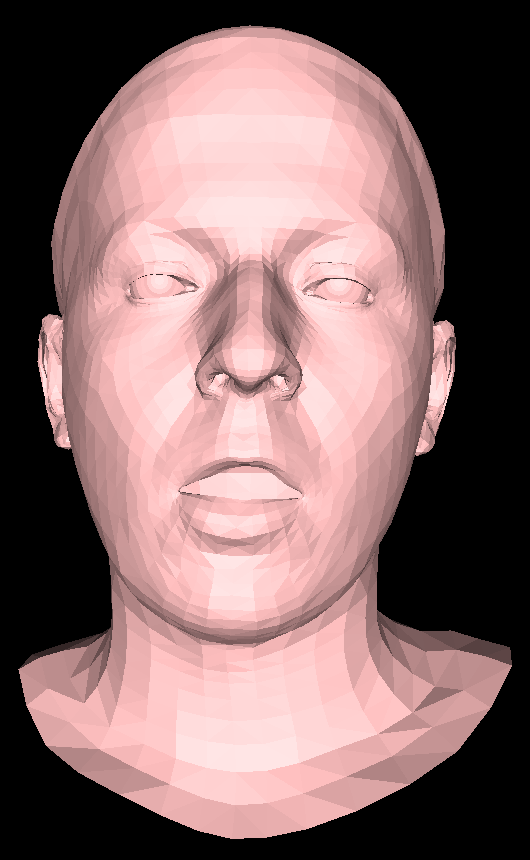
\includegraphics[width=\textwidth]{figures/voca_exp/vocaset_exp4.png}
    \end{subfigure}
    \begin{subfigure}[b]{0.19\textwidth}
        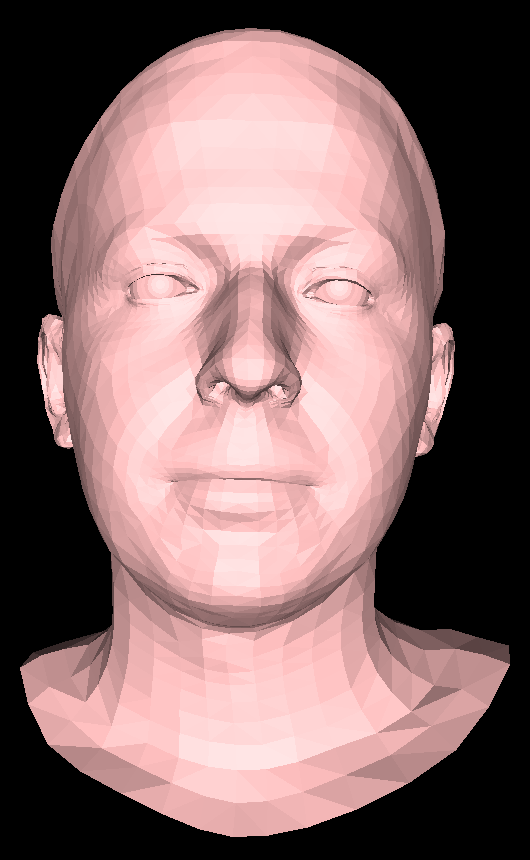
\includegraphics[width=\textwidth]{figures/voca_exp/vocaset_exp5.png}
    \end{subfigure}
    \caption{VOCASET Example Frames \cite{Cudeiro2019}}\label{fig:VOCASET_example}
\end{figure}

It should be noted that neither of these datasets were captured for the purpose of lip reading, but for synthesising realistic statistical facial models driven from an audio input, and thus there are no transcriptions for VOCASET.
The transcriptions could be obtained with an Audio Speech Recognition (ASR) method such as DeepSpeech \cite{Hannun2014} and then alignment would have to be performed to the datasets before using the data to train lip reading models.

\subsection{Lip Reading Models}
In \cite{Chung2016} Chung et al. used a multiple towers convolutional model based on the VGG-M architecture for multi-label classification to classify a video clip to one of the five hundred labels in the LRW dataset.
The model architecture (Figure \ref{fig:LRW_Multiple_Towers}) first processes each frame separately with a shared convolutional layer to extract features from each frame.
These features are down-sampled with a pooling layer before being concatenated into a single high channel feature map.
A one dimensional convolutional layer then reduces the channels of this feature map before being processed by subsequent convolutional and pooling layers.
The final layer of the model is passed through a softmax activation function \textcolor{red}{\textbf{(TO-DO add reference to softmax function)}} to predict one of the 500 word labels.

\begin{figure}[h]
    \centering
        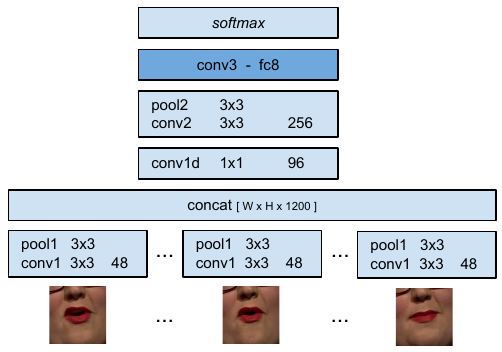
\includegraphics[width=0.7\textwidth]{figures/lrw_multiple_towers.png}
    \caption{LRW Multiple Towers Convolutional Neural Network Model \cite{Chung2016}}\label{fig:LRW_Multiple_Towers}
\end{figure}

Chung et al. suggest that the multiple towers model is effective due to the delay in time domain operations until after the first convolutional layer which allows for tolerance to registration errors in the dataset.

As well as measuring the performance of the model on total prediction accuracy, \cite{Chung2016} also use character-level edit distance, measured as the minimum number of characters required to be changed in the predicted label to obtain the ground truth.

The LipNet model \cite{Assael2016} was the first model produced to be able to predict end-to-end sentence-level lip reading of varied length, while previous work predicted on a word level.
The model used spatiotemporal convolutions to process multiple frames of video at once followed by a recurrent layer using Gated Recurrent Units (GRUs) \cite{Cho2014} and made character level predictions.
The model used the GRID dataset \cite{Cooke2006} due to it being the largest sentence level dataset at the time, on which LipNet achieved the state of the art performance.

As the LRW dataset could not be used to train a model such as LipNet for sentence-level lip reading, but the GRID dataset had limitations in the number of subjects and vocabulary, Chung et al. created the LRS dataset \cite{Chung2017}.
The model presented in \cite{Chung2017} was trained on both audio and video and made capable of taking either or both as the model inputs.
To prevent the model from being dependent on a single input source, the inputs are systematically distorted or removed.
The video input is passed through convolutional layers, followed by LSTM (Long Short-Term Memory) layers \cite{Cheng2016}, while the audio is converted to Mel-frequency cepstral coefficients (MFCC), then input to LSTM layers.
The two are combined with the attention mechanism and further LSTM layers and an output fully connected layer with softmax activation for character level predictions.
The model also makes use of curriculum learning by initially training the model on short sequences of single words, before the increasing the length of training sequences throughout training.
It is stated by \cite{Chung2017} that this accelerates training and reduces overfitting.

In 2018 DeepMind published their V2P (Video to Phonemes) model \cite{Shillingford2018} along with the LSVSR dataset built from content from YouTube. 
LSVSR greatly surpassed all previous datasets in size and variation, containing 3886 hours of training data.
The model follows a similar architecture to LipNet \cite{Assael2016} using spatiotemporal convolutional layers followed by recurrent layers, however it used an increased number of convolutional layers and used LSTM layers in place of than GRUs.
It should be commented that due to the size of the model and dataset dictated the use of 64 GPUs for training to allow a batch size of 128.
Unlike previous models, the V2P model predicts phonemes as opposed to characters, these phonemes are then processed by a language model for word prediction as with previous models.

To the best of the author's knowledge, there does not currently exist any papers which have explored the use of 3D temporal datasets for the use with lip reading models. 
This is likely due to the shortage of 3D temporal data due to the difficulties in obtaining such data, on which such models could be trained on.

\section{Data Generation}
In order to construct a deep learning lip reading model capable of being trained on 3D temporal data, appropriate datasets must first be established.
Existing datasets \cite{Tzirakis2019, Cudeiro2019} discussed in section \ref{3D Datasets} have been captured directly with the use of multi-camera capture rigs under controlled situations.
The total duration of both of these datasets is very short in comparison to the video datasets such as LRW, LRS and LSVSR, which is a limiting factor to the models which could be trained using them.

As the models also use different mesh models to represent the data that has been captured this also prevents the two datasets being joined directly.
Unlike video data, there currently lacks a large body of 3D video data which is publicly available, limiting the construction of 3D datasets to directly capturing more 3D scans with multi-camera capture rigs, similar to those used in \cite{Tzirakis2019, Cudeiro2019} and generating synthetic training data.

\subsection{Audio Driven Data Generation}
Karras et al. proposed a method for generating 3D facial animation from audio with the use of a CNN architecture \cite{Karras2017a}, see Figure \ref{fig:Karras_Model}.
The model is actor specific, but restricting this allowed fro the model to be trained on just 3-5 minutes of data per actor.
Firstly, a fixed function auto-correlation layer is used to extract a time-varying sequence of speech features from the audio input, named the formant analysis layer.
Then a five convolutional layers are used to extract short-term animation features from the formant analysis network layer.
This is then followed by five convolutional layers, with each input concatenated with a learned emotional state representation.
Finally two linear layers are used to drive vertex positions from a starting mesh of the given actor.

\begin{figure}[h]
    \centering
        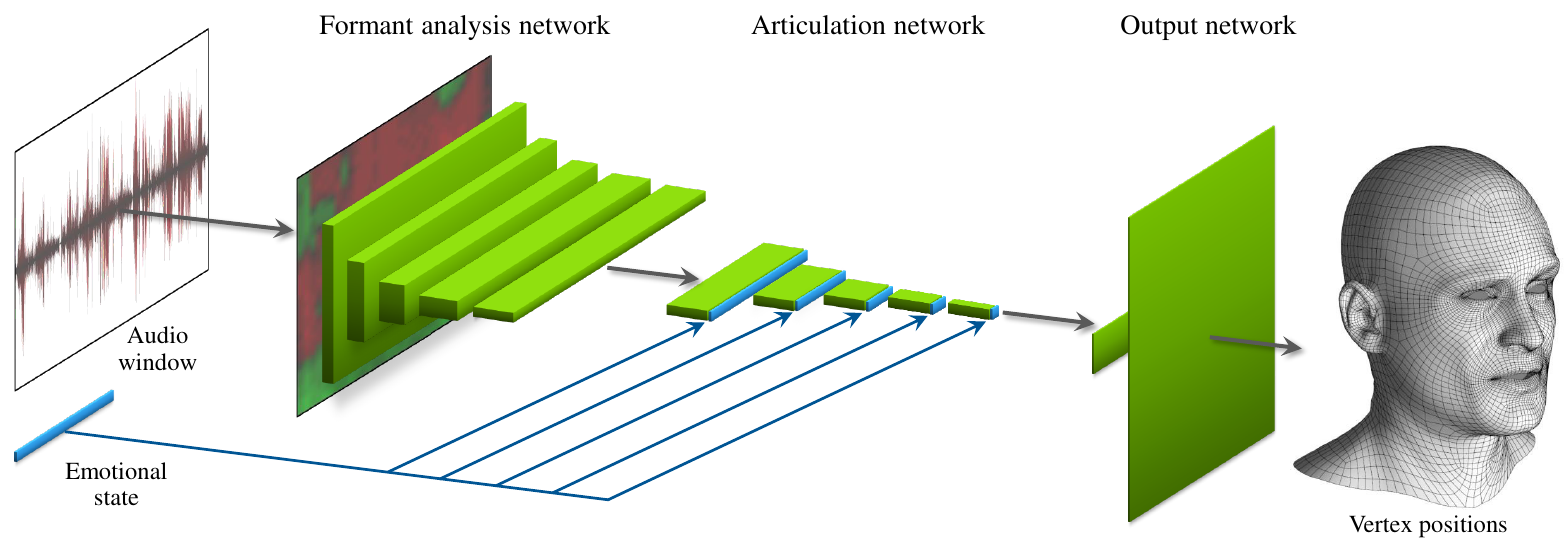
\includegraphics[width=0.9\textwidth]{figures/karras_model.png}
    \caption{Audio Driven Facial Animation Model Proposed by Karras et al. \cite{Karras2017a}}\label{fig:Karras_Model}
\end{figure}

However, as the model by Karras et al. is not independent of the actor it cannot generalise to new subjects.
Tzirakis et al. propose a model which is independent of speaker and capture rig \cite{Tzirakis2019}.
As discussed in section \ref{3D Datasets}, a dataset was constructed of 3D speaking faces using the LRW dataset \cite{Chung2016} for the corpus.
This allowed Tzirakis et al. to create a model which can synthesise facial motion from audio from the LRW dataset.
The model used is similar to that used in \cite{Karras2017a}, firstly extracting short term temporal features from the input audio with a convolutional network followed by another convolutional network to analyse the extracted features.
Unlike the model used in \cite{Karras2017a}, the model used in \cite{Tzirakis2019} is trained to drive learnt blendshapes as opposed to vertex positions.
This reduces the number of output parameters of the model substantially in comparison to that used by Karras et al while reducing the potential expressions possible to be produced by the model.

Similar to \cite{Tzirakis2019}, the VOCA model \cite{Cudeiro2019} synthesises video sequences of 3D models speaking given an audio input.
The VOCASET dataset discussed in section \ref{3D Datasets}, was captured with the intention of training this model to be independent of the speaker, hence a large range of speakers are used within the dataset.
The model is comprised of three sections: audio feature extraction, a feature encoder and a decoder to drive a template facial mesh from the FLAME model \cite{Li2017}.
The audio feature extraction makes use of the pre-trained Mozilla implementation of the DeepSpeech model, based on the paper by Hannun et al. \cite{Hannun2014}.
The DeepSpeech model takes audio as an input and returns the unnormalised log-probabilities for an alphabet of the 26 standard characters, a space, apostrophe and blank character for time slices in the audio input.
The encoder is a convolutional network which is conditioned on the speakers identity, such that the latent space of speaker styles can later be explored on new audio inputs.
Finally, the decoder is made up of a fully connected layer with a linear activation function is used to output the displacements of the 5023 vertices in the template face.
However, as the model is conditioned with the label of which speaker the input data is from, the model does not truly learn to generalise to multiple speakers, but learns each speaker separately, thus not being independent of the speaker.

\section{Summary of Related Literature}
Visual speech recognition has seen large improvements in recent years, progressing from word level prediction on a relatively small vocabulary set \cite{Chung2016}, to variable length sequences predicting a sequence at a sentence level with the use of recurrent networks making character level predictions to construct the completed sentence \cite{Shillingford2018}.
These advances have come in tandem with the increase in the size and variation of the datasets on which to train such models.
While there currently exist no datasets made up of 3D temporal data which have been constructed with the intention for lip reading, there has been progress in the area of 3D model generation from an audio input.
A proposed solution to this problem would be to generate synthetic 3D temporal data by using a generative model, allowing a VSR classifier to be trained on the resulting dataset.
The model by Karras et al. is currently not publicly available due to being researched in collaboration with Nvidia.
The VOCA model however, is publicly available, although how independent the model truly is of the speakers it was trained on is unclear.
The VOCA model also has additional dependencies on the DeepSpeech model and thus is not trained fully end-to-end, potentially losing some information which might be of use for driving facial animation.

%\bibliographystyle{unsrt}
%\bibliography{ref}
%\end{document}
